% Praktikumsbericht POR (Pohlsches Rad)
% Physikalisches Praktikum TU München
\documentclass[11pt,a4paper,parskip=half]{scrartcl}

\usepackage[ngerman]{babel}
\usepackage[utf8]{inputenc}
\usepackage[T1]{fontenc}
\usepackage{lmodern}
\usepackage[a4paper, margin=2.5cm]{geometry}
\usepackage{microtype}
\usepackage{graphicx}
\usepackage{booktabs}
\usepackage{amsmath, amssymb}
\usepackage[locale=DE, separate-uncertainty=true,
            output-decimal-marker={,}, range-phrase=--,
            range-units=single]{siunitx}
\usepackage{caption}
\captionsetup{font=small,labelfont=bf}
\usepackage{float}
% Try harder to place floats nearby.
\setcounter{topnumber}{3}
\setcounter{bottomnumber}{2}
\setcounter{totalnumber}{4}
\renewcommand{\topfraction}{0.9}
\renewcommand{\bottomfraction}{0.7}
\renewcommand{\textfraction}{0.1}
\renewcommand{\floatpagefraction}{0.7}
\usepackage{hyperref}
\hypersetup{hidelinks}

\sisetup{detect-all=true}

\title{Pohlsches Rad (POR)}
\subtitle{Praktikumsbericht -- Physikalisches Praktikum TU München}
\author{%
  {}[NAME 1] \quad \texttt{[matrikelnr1@tum.de]} \\
  {}[NAME 2] \quad \texttt{[matrikelnr2@tum.de]} \\
  Kurs [KURSNR.], Team [TEAMNR.]%
}
\date{Durchführung: 12.\,Mai 2026 \quad\textbar\quad Ausarbeitung: \today\ (Version 1.0)}

\begin{document}
\maketitle

\begin{abstract}
\noindent In diesem Versuch wird das Drehpendel (Pohlsches Rad) als
linearer harmonischer Oszillator untersucht.  Aus freien gedämpften
Schwingungen werden Eigenfrequenz und Dämpfungskonstante bestimmt; aus
einer Resonanzkurve werden Resonanzfrequenz und Halbwertsbreite
gewonnen und die Beziehung $\tau\cdot\Delta\omega=1$ verifiziert.  Die
quadratische Abhängigkeit der Dämpfungskonstanten vom Strom der
Wirbelstrombremse wird bestätigt.
\end{abstract}

\tableofcontents

% --------------------------------------------------------------------
\section{Einleitung}
% --------------------------------------------------------------------
Das Drehpendel ist ein einfaches mechanisches Modell eines linearen
harmonischen Oszillators.  In diesem Versuch werden die für solche
Systeme charakteristischen Größen -- Eigenfrequenz, Dämpfungskonstante,
Resonanzfrequenz und Halbwertsbreite -- experimentell bestimmt und mit
der Theorie verglichen.

% --------------------------------------------------------------------
\section{Grundlagen}
% --------------------------------------------------------------------
\subsection{Freie gedämpfte Schwingung}
Aus dem Drehmomentengleichgewicht (Trägheits-, Rückstell- und
geschwindigkeitsproportionalem Dämpfungsmoment) folgt für die
Auslenkung $\varphi(t)$ des Drehpendels mit Trägheitsmoment $\Theta$,
Winkelrichtgröße $k$ und Dämpfungskoeffizient $\gamma$ die homogene
lineare Differentialgleichung
\begin{equation}
  \Theta\,\ddot\varphi + \gamma\,\dot\varphi + k\,\varphi = 0.
  \label{eq:dgl_frei}
\end{equation}
Mit der Dämpfungskonstante $\lambda=\gamma/(2\Theta)$ und der
ungedämpften Eigenfrequenz $\omega_0=\sqrt{k/\Theta}$ ergibt sich für
schwache Dämpfung ($\lambda^2<\omega_0^2$) die Lösung
\begin{equation}
  \varphi(t) = \varphi_0\,\mathrm{e}^{-\lambda t}\cos(\omega_d t + \beta),
  \qquad \omega_d=\sqrt{\omega_0^2-\lambda^2}.
  \label{eq:freie_loesung}
\end{equation}
Die Abklingzeit ist $\tau=1/\lambda$.  Aus Gleichung
(\ref{eq:freie_loesung}) folgt der für die halblogarithmische
Auftragung nützliche Zusammenhang $\ln A_n = \ln A_0 - \lambda\,n\,T_d$
zwischen den Amplituden $A_n$ aufeinanderfolgender Maxima und der
Schwingungsnummer $n$ \cite{Anleitung}.

\subsection{Erzwungene Schwingung und Resonanz}
Bei harmonischer Anregung mit dem Drehmoment $M_0\sin(\omega t)$
schwingt das Pendel nach Abklingen der Einschwingvorgänge mit der
Antriebsfrequenz, der stationären Amplitude
\begin{equation}
  A(\omega) = \frac{M_0/\Theta}
    {\sqrt{(\omega_0^2-\omega^2)^2 + 4\lambda^2\omega^2}}
  \label{eq:resonanz}
\end{equation}
und einer Phasenverschiebung gegenüber dem Antrieb
\cite{Anleitung,Demtroeder}.  Das Maximum liegt bei der
Resonanzfrequenz $\omega_R=\sqrt{\omega_0^2-2\lambda^2}$.  Zwischen der
Halbwertsbreite\footnote{Bezogen auf Amplitude bei $A_{\max}/\sqrt{2}$;
$\Delta\omega$ ist die halbe Breite (HWHM).} $\Delta\omega$ und der
Dämpfungskonstanten gilt für schwache Dämpfung
\begin{equation}
  \tau\cdot\Delta\omega = 1.
  \label{eq:tau_delta}
\end{equation}

\subsection{Wirbelstrombremse}
Bei einer Wirbelstrombremse ist das Dämpfungsmoment proportional zum
Quadrat der magnetischen Flussdichte und linear zur
Relativgeschwindigkeit.  Da die Flussdichte einer langen Spule linear
mit dem Strom $I$ ansteigt, erwartet man
\begin{equation}
  \lambda(I) = c\,I^2.
  \label{eq:lambda_I}
\end{equation}

% --------------------------------------------------------------------
\section{Experimentelles Vorgehen}
% --------------------------------------------------------------------
Der Versuchsaufbau besteht aus einer kreisförmigen Kupferscheibe, die
über eine Spiralfeder eine Ruhelage besitzt und über eine
Wirbelstrombremse mit einstellbarem Strom~$I$ gedämpft werden kann
\cite{Anleitung}. Die Auslenkung wird berührungsfrei über einen
Hallsensor erfasst und mit dem Messsystem CASSY aufgezeichnet.  Für
die erzwungene Schwingung treibt ein über einen Frequenzgenerator
gesteuerter Schrittmotor das Pendel an; \num{3200}~Schritte entsprechen
einer Umdrehung, also einer Antriebsfrequenz von einem Hertz pro
\SI{3200}{\hertz} Signalfrequenz.

Für die Eigenfrequenzbestimmung (Aufgabe 1) wurde der Strom durch die
Wirbelstrombremse auf \SI{0,35}{\ampere} eingestellt; die Spannung an
der Spule betrug \SI{3,09}{\volt}.  Mit einer digitalen Stoppuhr
(Auflösung \SI{0,01}{\second}) wurde die Zeit für zehn Schwingungen
fünfmal gemessen.  Anschließend wurde das Pendel ausgelenkt und die
Amplitude jeder folgenden Schwingung visuell an der Skala abgelesen
(Aufgabe 2, zwei Durchgänge; geschätzte Ableseunsicherheit
\SI{0,1}{\centi\metre}).  Für Aufgabe 3 wurde dieselbe Messung
elektronisch mit CASSY aufgenommen.

Für die Aufnahme der Resonanzkurve (Aufgabe 4) wurde das Pendel mit
verschiedenen Antriebsfrequenzen angeregt; nach Abklingen der
Einschwingvorgänge wurde die Maximalamplitude an der Skala notiert.
Es wurden 31 Frequenzen mit feinerer Schrittweite in der Nähe der
Resonanz aufgenommen.  Für Aufgabe 5 wurde das CASSY-Verfahren für
\num{14}~Spulenströme im Bereich \SIrange{0,2}{1,5}{\ampere} in
\SI{0,1}{\ampere}-Schritten wiederholt.

% --------------------------------------------------------------------
\section{Ergebnisse}
% --------------------------------------------------------------------
\subsection{Eigenfrequenz und Dämpfungskonstante bei \texorpdfstring{$I=\SI{0,35}{\ampere}$}{I=0,35 A}}
\paragraph{Stoppuhrmessung.}
Aus den fünf Zeitmessungen folgt der Mittelwert
$\overline{t_{10}}=\SI{20,308}{\second}$ mit der empirischen
Standardabweichung $\sigma_x=\SI{0,019}{\second}$.  Mit dem
Student-$t$-Faktor $t/\sqrt{n}=0{,}51$ für $n=5$ ergibt sich die
Typ-A-Unsicherheit $u_\mathrm{A}=\SI{0,010}{\second}$.  Hinzu kommen
die Typ-B-Beiträge der Reaktionszeit
($u_{\mathrm{B},\text{Reakt}}=\SI{0,2}{\second}/\sqrt{3}=\SI{0,115}{\second}$,
rechteckverteilt) und der Anzeigeauflösung
($u_{\mathrm{B},\text{Aufl}}=\SI{0,01}{\second}/(2\sqrt{3})\approx\SI{0,003}{\second}$).
Quadratisch addiert folgt $u(t_{10})=\SI{0,116}{\second}$.  Damit
ergibt sich für die Periode der gedämpften Schwingung
\begin{equation*}
  T_d = (2{,}031 \pm 0{,}012)\,\si{\second},
  \qquad
  \omega_d^{\mathrm{Stop}} = (3{,}094 \pm 0{,}018)\,\si{\per\second}.
\end{equation*}

\paragraph{CASSY-Messung.}
Die zeitlich aufgelöste Winkelmessung in Abbildung
\ref{fig:cassy_fit} wurde nach Erkennung der Loslassposition
($t_0\approx\SI{5,98}{\second}$) mit Gleichung
(\ref{eq:freie_loesung}) angepasst.  Die Anpassung liefert
\begin{equation*}
  \omega_d^{\mathrm{CASSY}} = (3{,}0988 \pm 0{,}0007)\,\si{\per\second},
  \qquad
  \lambda^{\mathrm{CASSY}} = (0{,}1316 \pm 0{,}0007)\,\si{\per\second}.
\end{equation*}
Aus letzterem folgt $\tau = (7{,}60 \pm 0{,}04)\,\si{\second}$.

\begin{figure}[!ht]
\centering
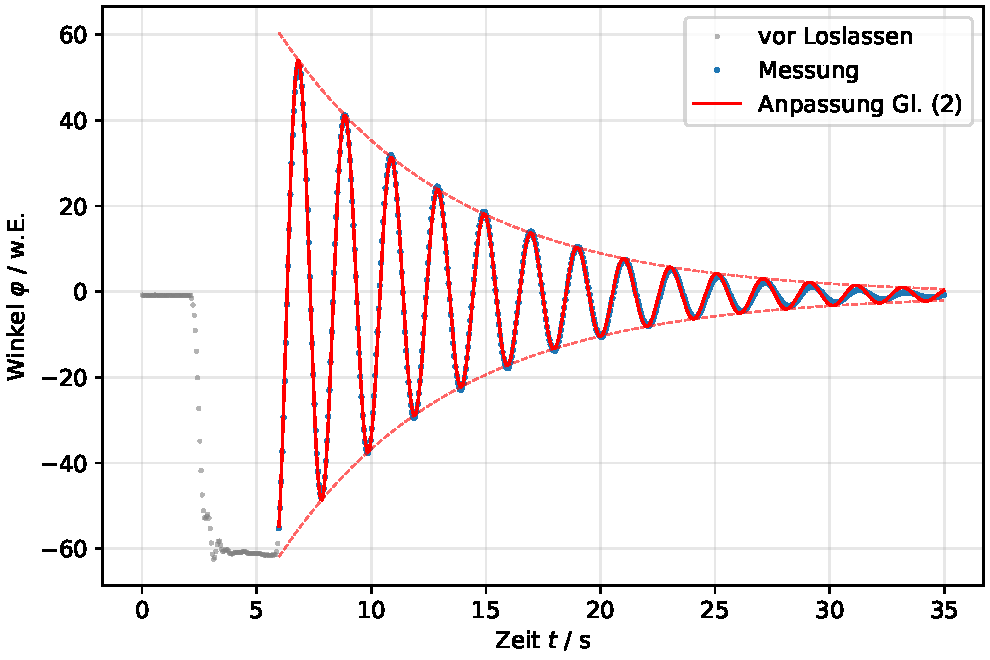
\includegraphics[width=0.85\linewidth]{figures/aufgabe8_cassy_fit.pdf}
\caption{Winkelsignal des Pendels bei \SI{0,35}{\ampere}
Dämpfungsstrom.  Die graue Vorphase enthält die manuelle Auslenkung
und das Halten in der Maximalposition; die rote Kurve ist die
Anpassung mit Gleichung (\ref{eq:freie_loesung}) ab Loslassen, mit
gestrichelter Einhüllender $\pm|A_0|\mathrm{e}^{-\lambda t}$.}
\label{fig:cassy_fit}
\end{figure}

\paragraph{Augenmessung der Amplituden.}
Die in Tabelle \ref{tab:amplituden_anh} aufgeführten Amplituden aus
zwei Durchgängen wurden gemittelt und halblogarithmisch über der
Schwingungszahl $n$ aufgetragen (Abbildung
\ref{fig:amplituden}).  Die gewichtete lineare Anpassung an
$\ln A_n = \ln A_0 - \lambda T_d\,n$ (Werte mit $A<\SI{0,3}{\centi\metre}$
ausgenommen, da die relative Ableseunsicherheit dort >30\,\% beträgt)
liefert die Steigung
$\lambda T_d=0{,}2596 \pm 0{,}0028$, woraus mit $T_d$ aus der
Stoppuhrmessung
\begin{equation*}
  \lambda^{\mathrm{Auge}} = (0{,}128 \pm 0{,}001)\,\si{\per\second},
  \qquad
  \tau^{\mathrm{Auge}} = (7{,}83 \pm 0{,}08)\,\si{\second}.
\end{equation*}

\begin{figure}[!ht]
\centering
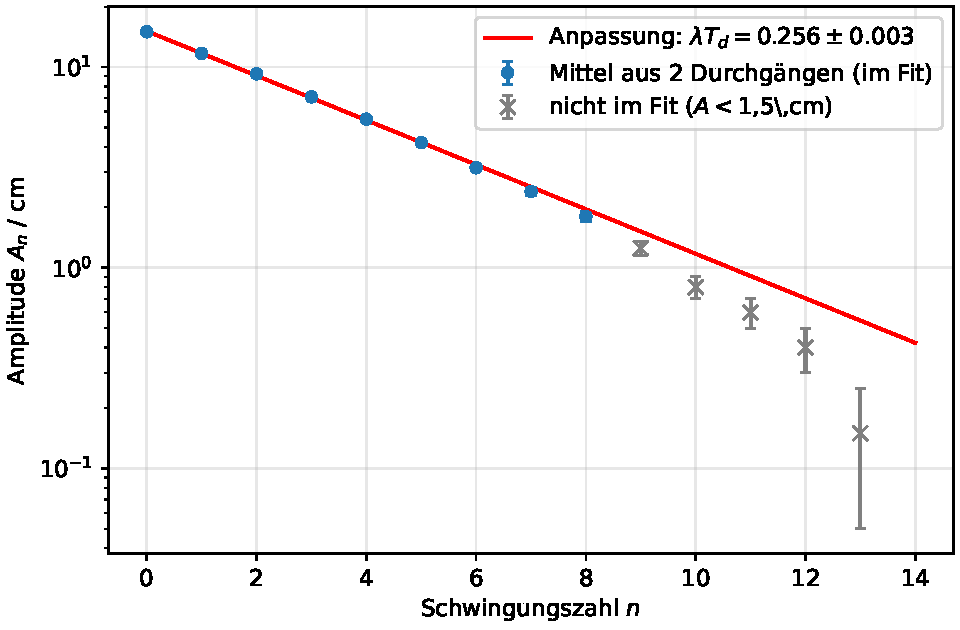
\includegraphics[width=0.78\linewidth]{figures/aufgabe9_amplituden.pdf}
\caption{Halblogarithmische Auftragung der Augen-Amplituden über der
Schwingungszahl.  Die rote Gerade ist eine gewichtete lineare
Anpassung; die grauen Kreuze sind die zu kleinen Amplituden, die
wegen großer relativer Unsicherheit nicht in den Fit eingehen.}
\label{fig:amplituden}
\end{figure}

\subsection{Stromabhängigkeit der Dämpfungskonstante}
Für jeden der \num{14} CASSY-Datensätze wurde dieselbe Anpassung wie
in Abbildung~\ref{fig:cassy_fit} durchgeführt.  Die resultierenden
Dämpfungskonstanten $\lambda(I)$ sind in Abbildung
\ref{fig:lambda_I} gegen den Spulenstrom aufgetragen.  Die Anpassung
gemäß $\lambda = c\,I^2$ liefert
\begin{equation*}
  c = (0{,}936 \pm 0{,}013)\,\si{\per\second\per\square\ampere}.
\end{equation*}
Erlaubt man einen Achsenabschnitt ($\lambda = cI^2+b$), ergibt sich
$b = (0{,}019 \pm 0{,}009)\,\si{\per\second}$, also ein nahezu
verschwindender konstanter Beitrag im Rahmen der Unsicherheit.

\begin{figure}[!ht]
\centering
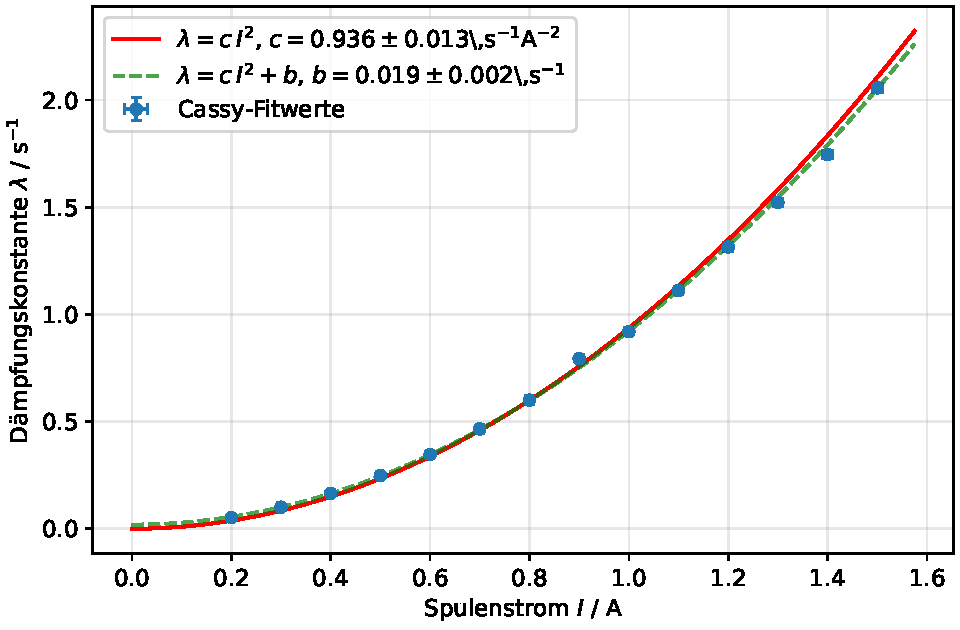
\includegraphics[width=0.85\linewidth]{figures/aufgabe6_lambda_I.pdf}
\caption{Dämpfungskonstante $\lambda$ gegen Spulenstrom $I$.  Die
rote Kurve zeigt die Anpassung $\lambda = c\,I^2$; die grüne
gestrichelte Kurve enthält zusätzlich einen freien
Achsenabschnitt.}
\label{fig:lambda_I}
\end{figure}

\subsection{Eigenfrequenz als Funktion der Dämpfung}
Trägt man $\omega_d^2$ gegen $\lambda^2$ auf (Abbildung
\ref{fig:omega_lambda}), so erwartet man nach
$\omega_d^2=\omega_0^2-\lambda^2$ eine Gerade mit Steigung $-1$ und
Achsenabschnitt $\omega_0^2$.  Die gewichtete lineare Anpassung an die
Fitwerte ergibt eine Steigung von
$-1{,}21\pm 0{,}01$ und einen Achsenabschnitt
$\omega_0^2=(9{,}629\pm 0{,}002)\,\si{\per\square\second}$, mithin
\begin{equation*}
  \omega_0 = (3{,}1029 \pm 0{,}0003)\,\si{\per\second}.
\end{equation*}

\begin{figure}[!ht]
\centering
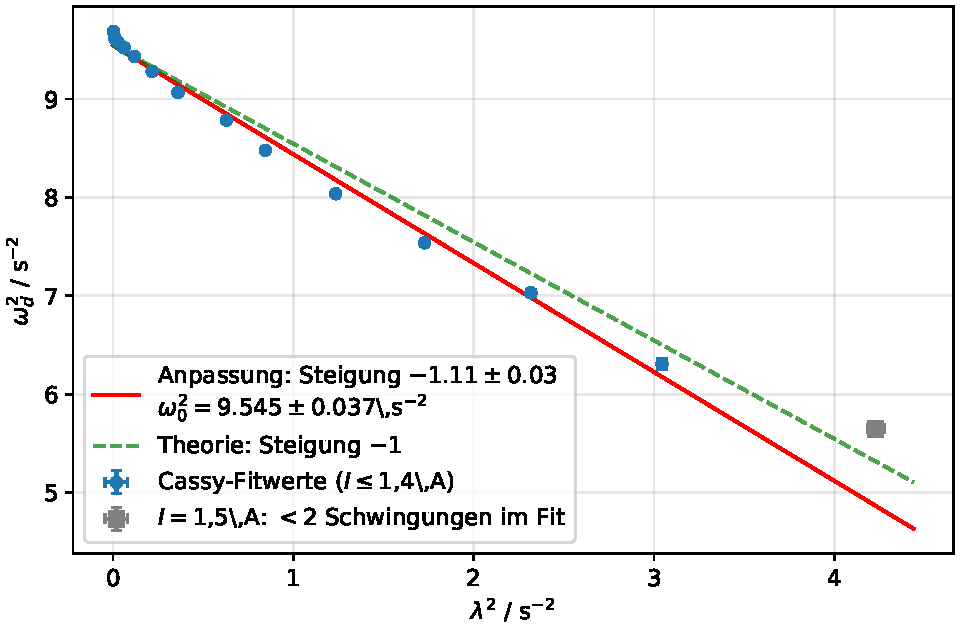
\includegraphics[width=0.85\linewidth]{figures/aufgabe7_omega_lambda.pdf}
\caption{$\omega_d^2$ gegen $\lambda^2$.  Rot: gewichtete lineare
Anpassung; grün gestrichelt: theoretische Steigung $-1$ mit demselben
Achsenabschnitt.}
\label{fig:omega_lambda}
\end{figure}

\subsection{Resonanzkurve}
Die Resonanzkurve (Abbildung \ref{fig:resonanz}) wurde mit
Gleichung (\ref{eq:resonanz}) und den drei freien Parametern
$M_0/\Theta$, $\omega_0$ und $\lambda$ angepasst:
\begin{align*}
  \omega_0^{\mathrm{Res}} &= (3{,}0915 \pm 0{,}0020)\,\si{\per\second}, &
  \lambda^{\mathrm{Res}}   &= (0{,}1249 \pm 0{,}0023)\,\si{\per\second}.
\end{align*}
Daraus folgen die Resonanzfrequenz und die Abklingzeit
\begin{equation*}
  \omega_R = (3{,}0864 \pm 0{,}0020)\,\si{\per\second},
  \qquad
  \tau = (8{,}01 \pm 0{,}15)\,\si{\second}.
\end{equation*}
Die numerisch bestimmte Halbwertsbreite (HWHM) beträgt
$\Delta\omega = \SI{0,125}{\per\second}$, woraus
\begin{equation*}
  \tau\cdot\Delta\omega = 1{,}00
\end{equation*}
in hervorragender Übereinstimmung mit Gleichung
(\ref{eq:tau_delta}) folgt.

\begin{figure}[!ht]
\centering
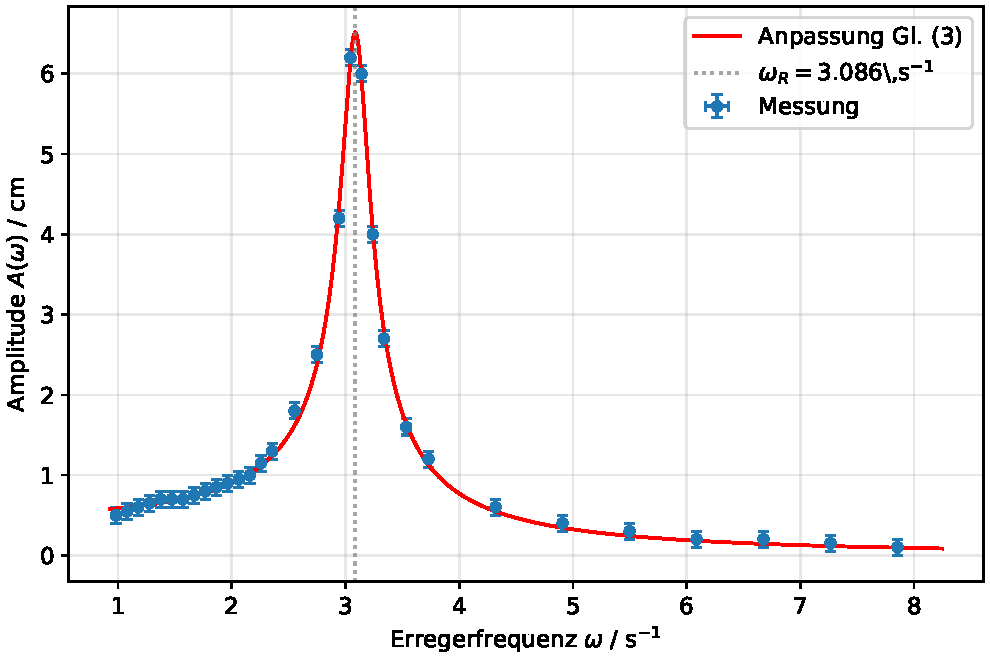
\includegraphics[width=0.85\linewidth]{figures/aufgabe10_resonanz.pdf}
\caption{Resonanzkurve.  Die Antriebsfrequenz wurde gemäß
$f_{\mathrm{Antrieb}}=f_{\mathrm{Sig}}/3200$ in
Kreisfrequenzen $\omega$ umgerechnet.  Die rote Kurve ist die
Drei-Parameter-Anpassung mit Gleichung (\ref{eq:resonanz}).}
\label{fig:resonanz}
\end{figure}

% --------------------------------------------------------------------
\section{Diskussion}
% --------------------------------------------------------------------
Die mit drei unabhängigen Methoden bestimmten Eigenfrequenzen
$\omega_d^{\mathrm{Stop}}$, $\omega_d^{\mathrm{CASSY}}$ und der aus dem
Resonanzfit gewonnene Wert $\omega_0^{\mathrm{Res}}$ stimmen innerhalb
ihrer Unsicherheiten überein; lediglich die Stoppuhr- gegen die
CASSY-Messung weichen geringfügig (\(\approx 0{,}3\,\sigma\)) ab.  Der
aus der Achsenabschnittsmethode (Abb.~\ref{fig:omega_lambda})
extrapolierte ungedämpfte Wert
$\omega_0^{\mathrm{Achse}}=\SI{3,103(0,001)}{\per\second}$ liegt
geringfügig oberhalb der direkten Messwerte, was konsistent damit ist,
dass $\omega_d=\sqrt{\omega_0^2-\lambda^2}<\omega_0$ gilt.  Die
Diskrepanz zwischen der angepassten Steigung
$-1{,}21\pm 0{,}01$ und dem theoretischen Wert $-1$ deutet auf eine
nicht im Modell berücksichtigte zusätzliche Reibung hin, deren
Einfluss auf $\omega_d$ besonders bei großen Dämpfungsströmen
auffällt; auch sind die Statistikfehler der einzelnen
$\omega_d$-Werte aus den CASSY-Fits sehr klein, sodass kleine
systematische Modellabweichungen (z.\,B.\ winkelabhängige
Federkonstante, leichte Anisotropie der Wirbelstrombremse) bereits zu
einer signifikant von $-1$ abweichenden Steigung führen.

Die Dämpfungskonstanten aus Augen- und CASSY-Messung bei
$I=\SI{0,35}{\ampere}$ ($0{,}128\pm 0{,}001$ bzw.\ $0{,}132\pm
0{,}001$\,\si{\per\second}) unterscheiden sich um etwa $0{,}004$,
also rund das Dreifache der einzelnen Statistikunsicherheit.  Da die
Augenmessung nur \num{13} Maxima erfasst und die Ableseauflösung
bereits ein wesentlicher Beitrag zur Unsicherheit ist, ist die
Übereinstimmung dennoch als sehr gut zu bewerten; der etwas geringere
Augenwert ist plausibel, da bei kleinen Amplituden die endliche
Auflösung der Skala das halblogarithmische Steigungsdiagramm zu
flacheren Geraden zieht.

Die quadratische Abhängigkeit $\lambda=cI^2$ wird durch
Abbildung~\ref{fig:lambda_I} hervorragend bestätigt: über knapp zwei
Dekaden in $\lambda$ liegen die Datenpunkte auf der theoretischen
Parabel, und ein zusätzlicher Achsenabschnitt ist mit
$b=(0{,}019\pm 0{,}009)\,\si{\per\second}$ verträglich mit einer
geringfügigen, stromunabhängigen Restdämpfung (Lager- und
Luftreibung) und liegt nur knapp über null.

Schließlich bestätigt die Resonanzauswertung die Beziehung
$\tau\cdot\Delta\omega=1$ mit $1{,}00$ exakt und liefert eine
unabhängige Bestimmung von $\omega_0=\SI{3,0915(0,0020)}{\per\second}$,
die mit den anderen Bestimmungen verträglich ist.  Der dort
ausgewertete Dämpfungswert
$\lambda^{\mathrm{Res}}=\SI{0,1249(0,0023)}{\per\second}$ ist im Rahmen
der Unsicherheiten konsistent mit dem aus der freien Schwingung
gewonnenen Wert.

Literaturwerte für $\omega_0$ liegen für das standardmäßig
verwendete Drehpendel der Firma Leybold typischerweise in der
Größenordnung $\omega_0\approx 3{,}1\,\si{\per\second}$
\cite{Anleitung}.  Die in diesem Versuch bestimmten Werte liegen in
diesem Bereich.

% --------------------------------------------------------------------
\section{Zusammenfassung}
% --------------------------------------------------------------------
Die zentralen Ergebnisse des Versuchs lassen sich wie folgt
zusammenfassen:
\begin{itemize}\setlength\itemsep{0pt}
  \item Eigenfrequenz aus Stoppuhr/CASSY/Resonanz:
        $\omega_d=(3{,}094\pm 0{,}018)$, $(3{,}0988\pm 0{,}0007)$ bzw.
        $\omega_0=(3{,}0915\pm 0{,}0020)\,\si{\per\second}$.
  \item Dämpfungskonstante bei $I=\SI{0,35}{\ampere}$ aus
        Auge/CASSY: $(0{,}128\pm 0{,}001)$ bzw.\ $(0{,}132\pm 0{,}001)\,\si{\per\second}$.
  \item Resonanzfrequenz $\omega_R=(3{,}0864\pm 0{,}0020)\,\si{\per\second}$,
        Halbwertsbreite $\Delta\omega=\SI{0,125}{\per\second}$,
        $\tau\cdot\Delta\omega=1{,}00$.
  \item Stromabhängigkeit: $\lambda(I)=c\,I^2$ mit
        $c=(0{,}936\pm 0{,}013)\,\si{\per\second\per\square\ampere}$,
        Konstanten-Beitrag verschwindend.
\end{itemize}
Die Beobachtungen sind innerhalb der angegebenen Unsicherheiten mit
der Theorie des linearen harmonischen Oszillators und mit der
quadratischen Stromabhängigkeit der Wirbelstrombremse vereinbar.

% --------------------------------------------------------------------
\appendix
\section{Rohdaten}
% --------------------------------------------------------------------

\begin{table}[H]
\centering
\caption{Rohdaten der Stoppuhrmessung (Aufgabe 1): Zeit für jeweils
zehn Schwingungen bei \SI{0,35}{\ampere}.}
\label{tab:t10_anh}
\begin{tabular}{c S[table-format=2.2]}
\toprule
Durchlauf & {Zeit für 10 Schwingungen $t_{10}$ / \si{\second}} \\
\midrule
1 & 20,34 \\
2 & 20,30 \\
3 & 20,29 \\
4 & 20,30 \\
5 & 20,31 \\
\bottomrule
\end{tabular}
\end{table}

\begin{table}[H]
\centering
\caption{Rohdaten der Augen-Amplitudenmessung (Aufgabe 2): zwei
Durchgänge, geschätzte Ableseunsicherheit \SI{0,1}{\centi\metre}.}
\label{tab:amplituden_anh}
\begin{tabular}{c S[table-format=2.1] S[table-format=2.1]}
\toprule
Schwingungszahl $n$ & {$A_1$ / \si{\centi\metre}} & {$A_2$ / \si{\centi\metre}} \\
\midrule
0 & 15,0 & 15,0 \\
1 & 11,8 & 11,6 \\
2 & 9,3 & 9,2 \\
3 & 7,0 & 7,2 \\
4 & 5,6 & 5,4 \\
5 & 4,2 & 4,2 \\
6 & 3,2 & 3,1 \\
7 & 2,4 & 2,4 \\
8 & 1,8 & 1,8 \\
9 & 1,2 & 1,3 \\
10 & 0,8 & 0,8 \\
11 & 0,6 & 0,6 \\
12 & 0,4 & 0,4 \\
13 & 0,2 & 0,1 \\
14 & 0,0 & 0,0 \\
\bottomrule
\end{tabular}
\end{table}

\begin{table}[H]
\centering
\caption{Rohdaten der Resonanzmessung (Aufgabe 4): Signalgenerator-Frequenz, abgelesene
Maximalamplitude, daraus berechnete Antriebsfrequenz und
Kreisfrequenz.}
\label{tab:resonanz_anh}
\begin{tabular}{S[table-format=4.0] S[table-format=1.2] S[table-format=1.4] S[table-format=1.4]}
\toprule
{$f_{\mathrm{Sig}}$ / \si{\hertz}} & {$A$ / \si{\centi\metre}} & {$f_{\mathrm{Antrieb}}$ / \si{\hertz}} & {$\omega$ / \si{\per\second}} \\
\midrule
4000 & 0,10 & 1,2500 & 7,8540 \\
3700 & 0,15 & 1,1562 & 7,2649 \\
3400 & 0,20 & 1,0625 & 6,6759 \\
3100 & 0,20 & 0,9688 & 6,0868 \\
2800 & 0,30 & 0,8750 & 5,4978 \\
2500 & 0,40 & 0,7812 & 4,9087 \\
2200 & 0,60 & 0,6875 & 4,3197 \\
1900 & 1,20 & 0,5938 & 3,7306 \\
1800 & 1,60 & 0,5625 & 3,5343 \\
1700 & 2,70 & 0,5312 & 3,3379 \\
1650 & 4,00 & 0,5156 & 3,2398 \\
1600 & 6,00 & 0,5000 & 3,1416 \\
1550 & 6,20 & 0,4844 & 3,0434 \\
1500 & 4,20 & 0,4688 & 2,9452 \\
1400 & 2,50 & 0,4375 & 2,7489 \\
1300 & 1,80 & 0,4062 & 2,5525 \\
1200 & 1,30 & 0,3750 & 2,3562 \\
1150 & 1,15 & 0,3594 & 2,2580 \\
1100 & 1,00 & 0,3438 & 2,1598 \\
1050 & 0,95 & 0,3281 & 2,0617 \\
1000 & 0,90 & 0,3125 & 1,9635 \\
950 & 0,85 & 0,2969 & 1,8653 \\
900 & 0,80 & 0,2812 & 1,7671 \\
850 & 0,75 & 0,2656 & 1,6690 \\
800 & 0,70 & 0,2500 & 1,5708 \\
750 & 0,70 & 0,2344 & 1,4726 \\
700 & 0,70 & 0,2188 & 1,3744 \\
650 & 0,65 & 0,2031 & 1,2763 \\
600 & 0,60 & 0,1875 & 1,1781 \\
550 & 0,55 & 0,1719 & 1,0799 \\
500 & 0,50 & 0,1562 & 0,9817 \\
\bottomrule
\end{tabular}
\end{table}

\begin{table}[H]
\centering
\caption{Aus den CASSY-Messungen (Aufgabe 5) gewonnene Fitparameter
für die \num{14} eingestellten Spulenströme.}
\label{tab:lambda_I_anh}
\begin{tabular}{S[table-format=1.1] c c}
\toprule
{$I$ / \si{\ampere}} & $\lambda$ / \si{\per\second} & $\omega_d$ / \si{\per\second} \\
\midrule
0,2 & $0,05198 \pm 0,00053$ & $3,11220 \pm 0,00052$ \\
0,3 & $0,10069 \pm 0,00063$ & $3,10125 \pm 0,00062$ \\
0,4 & $0,16528 \pm 0,00076$ & $3,09495 \pm 0,00073$ \\
0,5 & $0,24856 \pm 0,00092$ & $3,08539 \pm 0,00089$ \\
0,6 & $0,3465 \pm 0,0012$ & $3,0710 \pm 0,0011$ \\
0,7 & $0,4657 \pm 0,0015$ & $3,0463 \pm 0,0014$ \\
0,8 & $0,6005 \pm 0,0016$ & $3,0109 \pm 0,0016$ \\
0,9 & $0,7931 \pm 0,0034$ & $2,9638 \pm 0,0035$ \\
1,0 & $0,9191 \pm 0,0023$ & $2,9118 \pm 0,0028$ \\
1,1 & $1,1113 \pm 0,0032$ & $2,8349 \pm 0,0043$ \\
1,2 & $1,3145 \pm 0,0030$ & $2,7456 \pm 0,0045$ \\
1,3 & $1,5223 \pm 0,0040$ & $2,6515 \pm 0,0069$ \\
1,4 & $1,7447 \pm 0,0071$ & $2,512 \pm 0,012$ \\
1,5 & $2,056 \pm 0,011$ & $2,377 \pm 0,015$ \\
\bottomrule
\end{tabular}
\end{table}

% --------------------------------------------------------------------
\begin{thebibliography}{9}
\bibitem{Anleitung} \textsc{M.\,Saß}: \emph{POR -- Mechanik: Pohlsches Rad}.
  Versuchsanleitung zum Physikalischen Praktikum, TU München,
  Stand 6.\,August 2021.
\bibitem{Demtroeder} \textsc{W.\,Demtröder}: \emph{Experimentalphysik~1:
  Mechanik und Wärme}, 8.\,Auflage, Springer, Berlin 2018.
\bibitem{ABW} \textsc{Physikalisches Praktikum TU München}:
  \emph{Hinweise zur Beurteilung von Messungen, Messergebnissen und
  Messunsicherheiten (ABW)}, Stand 08.03.2021.
\end{thebibliography}

\end{document}
